\chapter{Implémentation \& Conception}

\section{Système d'accouplement fourche–T}

\subsection{Principe de fonctionnement}

L'accouplement entre la tige du mouvement horloger et l'arbre moteur est réalisé au moyen d'un système à ergots de type fourche–T. 
D'un côté, une pièce en forme de T solidaire de l'arbre moteur vient s'engager dans une fourche à deux ergots espacés de 25 mm, montée sur la tige du mouvement. 
Ce principe d'accouplement à jeu angulaire transmet le couple de rotation tout en découplant les axes radiaux : les forces parasites susceptibles d'endommager le mouvement (charges radiales, bending) ne sont pas transmises, et une certaine tolérance au désalignement angulaire et radial est assurée naturellement par le jeu entre les ergots et le T.

\subsection{Analyse de la saccade due au désalignement}

En revanche, un désalignement résiduel entre les deux axes introduit une variation périodique du rapport de transmission instantané, se traduisant par une légère saccade superposée au profil de vitesse théorique. 
Pour un profil trapézoïdal 1/3–1/3–1/3 (accélération, vitesse constante, décélération), cette saccade se manifeste principalement en début et en fin de mouvement, là où la dérivée de vitesse est non nulle. 
Afin de maintenir l'erreur de vitesse en dessous de 5 \%, le défaut d'alignement radial maximal admissible doit être rigoureusement contrôlé lors du montage.

\subsubsection{Profil de vitesse avec saccade de désalignement}

La \autoref{fig:profil_saccade} illustre la superposition de la saccade périodique sur le profil de vitesse trapézoïdal théorique pour un accouplement fourche–T. 
Le désalignement radial a été dimensionné pour que l'erreur de vitesse n'excède jamais 5 \%.

\begin{figure}[H]
  \centering
  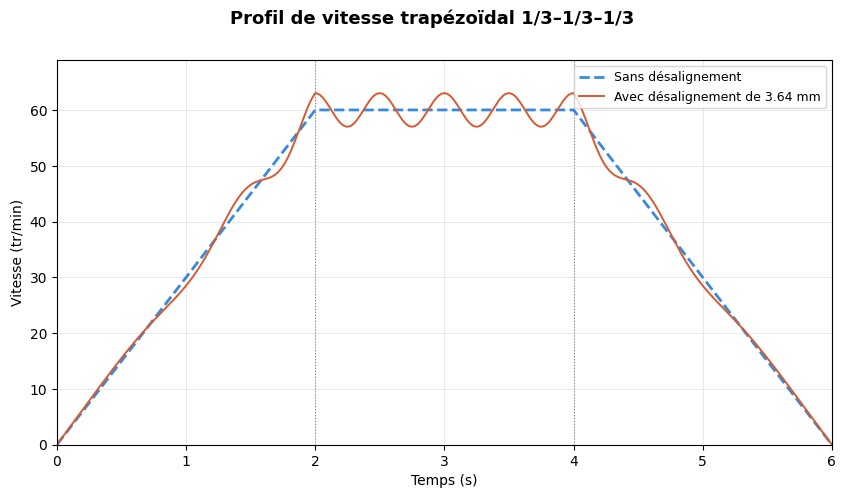
\includegraphics[width=0.85\textwidth]{assets/figures/Implementation/profil de vitesse trapezoidale avec saccade.png}
  \caption{Profil de vitesse trapézoïdal 1/3–1/3–1/3 avec saccade périodique due au désalignement de l'accouplement fourche–T.}
  \label{fig:profil_saccade}
\end{figure}

\subsubsection{Dimensionnement du désalignement maximal admissible}

La relation reliant l'erreur relative de vitesse $\varepsilon$ au désalignement $e$ et au rayon effectif $R_{\text{eff}}$ est donnée par :

\[
  \varepsilon_{\text{max}} = \frac{e^2}{2R_{\text{eff}}^2} \times 100\ (\%)
\]

En inversant cette formule, on obtient le désalignement maximal admissible pour un seuil d'erreur de 5 \% et un rayon effectif $R_{\text{eff}} = 11{,}5\ \text{mm}$ :

\[
  e_{\text{max}} = R_{\text{eff}} \sqrt{2 \cdot \frac{\varepsilon_{\text{seuil}}}{100}} = 11{,}5 \times \sqrt{2 \times 0{,}05} \approx 3{,}64\ \text{mm}
\]

\subsubsection{Analyse des tolérances de montage entre mouvements}

Les différents mouvements n'ayant pas les mêmes dimensions la hauteur de la tige peut varier lors du montage dépendamment du mouvement.
\begin{align*}
  \text{Mouvement 1} &: 8{,}73 - 4{,}1 = 4{,}63\ \text{mm} \\
  \text{Mouvement 2} &: 7{,}23 - 2{,}8 = 4{,}43\ \text{mm} \\
  \text{Mouvement 3} &: 6{,}63 - 2{,}2 = 4{,}43\ \text{mm} \\
  \text{Mouvement 4} &: 8{,}63 - 4{,}2 = 4{,}43\ \text{mm} \\
  \text{Mouvement 5} &: 3{,}80 - 1{,}5 = 2{,}30\ \text{mm} \\
  \text{Mouvement 6} &: 3{,}05 - 1{,}0 = 2{,}05\ \text{mm} \\
  \text{Mouvement 7} &: 9{,}33 - 4{,}1 = 5{,}23\ \text{mm}
\end{align*}

La différence entre la hauteur maximale (Mouvement 7 : $5{,}23\ \text{mm}$) et minimale (Mouvement 6 : $2{,}05\ \text{mm}$) s'élève à :

\[
  \Delta h = 5{,}23 - 2{,}05 = 3{,}18\ \text{mm}
\]

Cette variation de \SI{3.18}{\mm} entre les différents mouvements étant inférieur au \SI{3.64}{\mm} de désalignement acceptable pour ne pas dépasser les 5 \% d'erreur, cette méthode de montage ne constitue donc pas un problème majeur pour le système.

\subsection{Analyse des contraintes et déformations}

\subsubsection{Données du problème}

La masse rapportée en bout de tige est un cylindre de fonte grise ($\rho = 7{,}2\ \text{g/cm}^3$) d'un volume de $825{,}35\ \text{mm}^3$, ce qui donne une masse de :

\[
  m = \rho \cdot V = 7{,}2 \times 10^{-3} \times 825{,}35 \times 10^{-3} = 5{,}94\ \text{g}
\]

La tige est modélisée comme une poutre encastrée-libre en acier inoxydable ($E = 200\ \text{GPa}$), de diamètre $d = 1{,}2\ \text{mm}$ et de longueur $L = 10{,}75\ \text{mm}$.

\subsubsection{Propriétés de la section transversale}

Le moment quadratique et le module de résistance d'une section circulaire pleine sont :

\[
  I = \frac{\pi d^4}{64} = \frac{\pi \times 1{,}2^4}{64} \approx 0{,}1018\ \text{mm}^4
  \qquad
  W = \frac{\pi d^3}{32} \approx 0{,}1696\ \text{mm}^3
\]

\subsubsection{Efforts générés}

La force appliquée en bout correspond au poids de la masse :

\[
  F = m \cdot g = 5{,}94 \times 10^{-3} \times 9{,}81 \approx 58{,}3\ \text{mN}
\]

Le moment fléchissant maximal, situé à l'encastrement, vaut :

\[
  M_{max} = F \cdot L = 58{,}3 \times 10^{-3} \times 10{,}75 \approx 0{,}627\ \text{N{\cdot}mm}
\]

\subsubsection{Flèche en bout de tige}

En appliquant la formule de la poutre encastrée chargée en bout :

\[
  f = \frac{F L^3}{3EI}
  = \frac{58{,}3 \times 10^{-3} \times 10{,}75^3}{3 \times 200\,000 \times 0{,}1018}
  \approx 3{,}8 \times 10^{-3}\ \mu\text{m}
\]

La déflexion est donc de l'ordre du \textbf{nanomètre}, ce qui est négligeable au regard de toute tolérance mécanique en horlogerie.

\subsubsection{Contrainte de flexion}

La contrainte normale maximale, à l'encastrement, est :

\[
  \sigma_{max} = \frac{M_{max}}{W} = \frac{0{,}627}{0{,}1696} \approx 3{,}7 \times 10^{-3}\ \text{MPa}
\]

La limite élastique d'un acier inoxydable courant étant de l'ordre de $300\ \text{MPa}$, la marge de sécurité est supérieure à $\times 80\,000$. La tige ne présente \textbf{aucun risque de déformation plastique}.
